\documentclass[12pt]{article}
\usepackage{amsmath, amssymb, amsthm}
\usepackage{mathtools}
\usepackage{graphicx}
\usepackage{float}
\usepackage{hyperref}
\usepackage{xcolor}
\usepackage{listings}
\usepackage{geometry}
\usepackage{algorithm}
\usepackage{algpseudocode}
\usepackage{tikz}
\usepackage{longtable}

\usetikzlibrary{matrix}
\lstset{
  basicstyle=\ttfamily,
  frame=single,
  breaklines=true,
  xleftmargin=2em,
  tabsize=4
}
% Page Setup
\geometry{a4paper, margin=1in}

% Title Section
\title{\textbf{Eigenvalue Computation of Complex Matrices}}
\author{Agamjot Singh\\EE24BTECH11002\\IIT Hyderabad}
\date{\today}
\numberwithin{equation}{section}

\newcommand{\vecb}[1]{\mathbf{#1}}
\newcommand{\brak}[1]{\ensuremath{\left(#1\right)}}
\newcommand{\cbrak}[1]{\ensuremath{\left\{#1\right\}}}
\newcommand{\defmat}[2]{#1\in\mathbb{C}^{#2\times#2}}
\newcommand{\defvec}[2]{\vecb{#1}\in\mathbb{C}^{#2}}
\newcommand{\abs}[1]{\left\vert#1\right\vert}
\newcommand{\norm}[1]{\left\lVert#1\right\rVert}

\begin{document}

\maketitle

\begin{abstract}
This report presents an efficient algorithm for finding the eigenvalues of matrices with complex entries using a combination of Householder transformations and QR decomposition \brak{\text{via Givens rotation algorithm}}. The implementation is in C, and we discuss the theory and the approach taken.
\end{abstract}

\section{Introduction}
Finding eigenvalues of complex matrices is a critical task in various scientific and engineering applications. This report explores an efficient approach using a combination of:
\begin{itemize}
    \item \textbf{Householder Transformations:} to reduce the matrix to Hessenberg form.
    \item \textbf{Givens Rotations:} for QR decomposition of the Hessenberg matrix.
\end{itemize}

\section{Theory}
We start off by defining some basic concepts that we will be using throughout:
\subsection{Eigenvectors and Eigenvalues}
When we multiply a vector $\defvec{v}{m}$, $\vecb{v} \neq \vecb{0}$ by a matrix $\defmat{A}{m}$ we get a resultant vector $\vecb{x} = A\vecb{v}$, $\defvec{x}{m}$. This transformation rotates, stretches, or shears the vector $\vecb{v}$. Now we choose the vector $\vecb{v}$ such that this linear transformation only stretches, with no rotation or shear.
This chosen vector is the \textbf{eigenvector} of the matrix $A$. The corresponding \textbf{eigenvalue} is defined as the factor by which the eigenvector has been stretched.
\newline
Mathematically speaking,
\begin{align}
\label{eigen:1}
    A\vecb{v} = \lambda\vecb{v}
\end{align}
where $\vecb{v}$ is the eigenvector and $\lambda \in \mathbb{C}$ is the corresponding eigenvalue.
\newline

Equation \brak{\ref{eigen:1}} can also be stated as,
\begin{align}
\label{eigen:2}
   \brak{A - \lambda I} \vecb{v} = \vecb{0} 
\end{align}
where $I \in \mathbb{C}^{m \times m}$ is the identity matrix of order $m$.
\newline

Equation \brak{\ref{eigen:2}} has non zero solution $\vecb{v}$ if and only if, 
\begin{align}
\label{eigen:3}
    \text{det}\brak{A - \lambda I} = 0
\end{align}

\subsection{Similarity Transformation}
A similarity transformation on a matrix $\defmat{A}{m}$ with transformation matrix $\defmat{A^{\prime}}{m}$ is given by,
\begin{align}
    A^{\prime} = X^{\ast} A X
\end{align}
where $X$ is a unitary matrix and $X^{\ast}$ is the conjugate transpose of $X$.
Note that, for $X$ to be unitary, it satisfies,
\begin{align}
    \label{sim:2}
    X^{\ast}X = XX^{\ast} = I
\end{align}

We will now show that a similarity transformation preserves the eigenvalues of any matrix.
\newline
Say $\lambda^{\prime} \in \mathbb{C}$ is an eigenvalue of the matrix $A^{\prime}$, hence by equation \brak{\ref{eigen:3}} and \brak{\ref{sim:2}},
\begin{align}
    \text{det}\brak{A^{\prime} - \lambda^{\prime} I} &= 0\\
    \text{det}\brak{X^{\ast}AX - \lambda^{\prime} X^{\ast}X} &= 0\\
    \text{det}\brak{X^{\ast}\brak{A - \lambda^{\prime}I} X} &= 0\\
    \label{sim:3} \implies \text{det}\brak{X^{\ast}} \text{det}\brak{A - \lambda^{\prime}I} \text{det}\brak{X} &= 0\\
\end{align}
From equation \brak{\ref{sim:2}}, $X$ is invertible with $X^{-1} = X^{\ast}$. Hence $\text{det} \brak{X} = \frac{1}{\text{det} \brak{X^{\ast}}}\neq 0$.
\newline
Using this fact in equation \brak{\ref{sim:3}}, we get,
\begin{align}
    \text{det}\brak{A - \lambda^{\prime} I} = 0
\end{align}

This proves that eigenvalues of $A^{\prime}$ are exactly same as the eigenvalues of $A$. Similarily, it can also be proved that eigenvalues of $A$ are same as that of $A^{\prime}$.
\newline
Similarily transformations are the basic building block of computing eigenvalues efficiently which will be extensively used in this implementation.

\subsection{QR decomposition} \label{qrth}
$QR$ decomposition is a decomposition of a matrix $\defmat{A}{m}$ into a product $A = QR$, such that $\defmat{Q}{m}$ is an square unitary matrix with all of its columns having unit norm and $\defmat{R}{m}$ is an upper triangular matrix. 
\newline
\newline
Geometrically speaking, the matrix $A$ can be thought of as a set of vectors \brak{\text{columns of } A} in the $m$-dimensional space.
The matrix $Q$ represents an orthonormal basis for the column space of $A$. It "replaces" the original vectors of $A$ with a new set of orthonormal vectors.
The matrix $R$ provides the coefficients needed to express the original vectors of $A$ as linear combinations of the new orthonormal vectors in $Q$.

\section{Pros and Cons of Householder transformation and Givens rotation}
\subsection{Time complexity}
\begin{itemize}
    \item Householder reflections: $O\brak{n^3}$
    \item Givens rotations for QR decomposition: $O\brak{n^3}$ for dense matrices, $O\brak{n}$ per rotation (efficient for sparse matrices).
    \item Total: $O\brak{n^3}$
\end{itemize}

\subsection{Numerical Stability}
\begin{itemize}
    \item High stability due to orthogonal transformations.
\end{itemize}

\subsection{Applicability}
\begin{itemize}
    \item Suitable for dense matrices.
    \item Can handle both real and complex matrices effectively.
\end{itemize}


\subsection{Memory Usage}
\begin{itemize}
    \item Moderate, requires storing Householder vectors and applying Givens rotations in place.
\end{itemize}

\begin{longtable}{|p{2.5cm}|p{3.5cm}|p{3.5cm}|p{2.5cm}|p{2.5cm}|}
\hline
\textbf{Algorithm} & \textbf{Pros} & \textbf{Cons} & \textbf{Time Complexity} & \textbf{Conditions} \\ \hline
\endfirsthead
\hline
\textbf{Algorithm} & \textbf{Pros} & \textbf{Cons} & \textbf{Time Complexity} & \textbf{Conditions} \\ \hline
\endhead
Householder + Givens & Stable, precise; preserves sparsity. & Complex preprocessing for Hessenberg form. & \( O(n^3) \) & Any square matrix. \\ \hline
Jacobi Method & Accurate for symmetric matrices; simple. & Slow for non-symmetric matrices; inefficient for large ones. & \( O(n^3) \) (dense) & Symmetric (real/complex). \\ \hline
Lanczos Algorithm & Efficient for sparse symmetric matrices. & Sensitive to rounding; limited to Hermitian matrices. & \( O(kn^2) \) & Sparse, symmetric/Hermitian. \\ \hline
QR Algorithm & Robust for eigenvalue computation. & High cost for large dense matrices. & \( O(n^3) \) & Any square matrix. \\ \hline
Arnoldi Algorithm & Handles non-symmetric sparse matrices. & Requires re-orthogonalization; less stable. & \( O(kn^2) \) & Sparse, any matrix. \\ \hline
Power Iteration & Simple, finds dominant eigenvalue. & Only computes the largest eigenvalue; slow for close eigenvalues. & \( O(kn^2) \) & Any square matrix. \\ \hline
\end{longtable}

\subsection{Why did we choose this particular algorithm?}
\begin{itemize}
\item Stability: It offers high numerical stability, making it suitable for dense, symmetric matrices.
\item Efficient Hessenberg Reduction: Householder transforms reduce the matrix to Hessenberg form, simplifying eigenvalue calculations.
\item Orthogonality: Maintains orthogonality during transformations, preserving accuracy.
\item Full Spectrum Calculation: Efficient for computing all eigenvalues, especially in iterative methods like QR iteration.
\item Numerically Robust: Handles ill-conditioned matrices better than simpler methods like Power Iteration.
\end{itemize}

\section{Algorithm Overview}
\textbf{First of all, why not just take the determinant of the matrix and find the roots of} $\text{det}\brak{A - \lambda I} = 0$ \textbf{?}
\newline
Well, it's $O\brak{m!}$, and that speaks for itself. It will blow up with extreme rates with increasing $m$.
\newline
Therefore, we employ a multi-step approach to find the eigenvalues of a complex matrix $\defmat{A}{m}$:

\subsection{The Basic QR Algorithm - Schur Decomposition}
In this algorithm, a sequence of matrices $\cbrak{A_k}$, $\defmat{A_k}{m}$ is generated iteratively, converging towards an upper triangular matrix. Under specific conditions, the convergence of off-diagonal elements follows a rate based on the ratio of eigenvalues.

As discussed in section $\ref{qrth}$, any matrix $A_k$ can be expressed as,
\begin{align}
    A_k = Q_k R_k
\end{align}
where $Q_k^{\ast}Q_k = I$.
\newline
Now we take $A_{k+1}$ such that,
\begin{align}
    A_{k + 1} = R_k Q_k = Q_k^{\ast} A_k Q_k
\end{align}
We can observe that the above transformation is a similarity transformation. Hence the eigenvalues of any matrix in the sequence $\cbrak{A_k}$ are identical.
\newline
The matrix sequence $\cbrak{A_k}$ converges \brak{\text{although very slowly in its current form}} towards an upper triangular matrix, with its eigenvalues as diagonal elements.
This algorithm computes an upper triangular matrix $T$ and a unitary matrix $U$ such that $A = UTU^{\ast}$ is the Schur decomposition of $A$.

\begin{align}
    A_k = Q_k^{\ast} A_{k - 1} Q_k = Q_k^{\ast} Q_{k - 1}^{\ast} A_{k - 2} Q_{k - 1} Q_k = \dots = Q_k^{\ast}\dots Q_1^{\ast} A Q_1 \dots Q_k
\end{align}
We can observe that $U_k = Q_1 Q_2 Q_3 \dots Q_k$, and $U = U_{\infty}$.
Also note that $T = A_{\infty}$.

Let the eigen values of $A$ be $\lambda_1$, $\lambda_2$, $\lambda_3 \dots \lambda_m$, such that
\begin{align}
    \abs{\lambda_1} \geq \abs{\lambda_2} \geq \abs{\lambda_3} \dots \geq \abs{\lambda_m}
\end{align}
We state, without proof, that the subdiagonal elements of $A$ converge like
\begin{align}
    \abs{a_{ij}^{\brak{k}}} = O\brak{\abs{\frac{\lambda_i}{\lambda_j}}^k}, i > j
\end{align}

\subsection{Householder Transformations to Hessenberg form}
As stated before, the vanilla $QR$ algorithm converges very slowly without any tweaking involved.
One such tweak is reducing the matrix to a hessenberg matrix form using similarity transforms and then apply the $QR$ algorithm. 
This is achieved by Householder Transformations on the original matrix to convert it into hessenberg form.
\newline
Note that a Hessenberg matrix is of the form,
\begin{align}
H = \begin{bmatrix}
\times & \times & \times & \times & \times\\
\times & \times & \times & \times & \times\\
0 & \times & \times & \times & \times\\
0 & 0 & \times & \times & \times\\
0 & 0 & 0 & \times & \times
\end{bmatrix}   
\end{align}
\subsubsection{Householder reflectors}
A Householder reflector matrix is of the form
\begin{align}
    P = I - 2\vecb{u}\vecb{u}^{\ast}
\end{align}
where $\defmat{P}{m}$ and $\defvec{u}{m}$, $\norm{\vecb{u}} = 1$.

Note that Householder reflectors are Hermitian, i.e. $P^{\ast} = P$ and $P^2 = I$. As $P^{\ast}P = I$, we also come to the conclusion
that $P$ is a unitary matrix.
\newline
We want the Householder reflector to transform any vector $\defvec{x}{m}$ to a multiple of $\vecb{e_1}$, where $\vecb{e_n}$ is the impulse vector with $n = 1$.
\begin{align}
\label{hhr:1}
    P\vecb{x} = \vecb{x} - 2\vecb{u}\brak{\vecb{u^{\ast}}\vecb{x}} = \alpha \vecb{e_1}
\end{align}
Since $P$ is unitary, $\norm{P\vecb{x}} = \norm{\vecb{x}}$.
\newline
Hence by taking norm on both sides on equation \brak{\ref{hhr:1}}, we get $\abs{\alpha} = \norm{\vecb{x}}$. Therefore, $\alpha = \rho\norm{\vecb{x}}$, where $\rho \in \mathbb{C}$, $\abs{\rho} = 1$. 
\newline
By rearranging equation \brak{\ref{hhr:1}},
\begin{align}
    \vecb{x} - \rho\norm{\vecb{x}}\vecb{e_1} = 2\vecb{u}\brak{\vecb{u^{\ast}}\vecb{x}}
\end{align}
As $\vecb{u}$ is unit norm,
\begin{align}
\label{hhr:2}
    \vecb{u} = \frac{\vecb{x} - \rho\norm{\vecb{x}}\vecb{e_1}}{\norm{\vecb{x} - \rho\norm{\vecb{x}}\vecb{e_1}}} = \frac{1}{\norm{\vecb{x} - \rho\norm{\vecb{x}}\vecb{e_1}}} \begin{pmatrix} x_1 - \rho\norm{\vecb{x}}\\x_2\\\vdots\\x_n\end{pmatrix}
\end{align}
Selection of $\rho$ is flexible as long as $\abs{\rho} = 1$. To ease out the process, we take $\rho = \frac{x_1}{\abs{x_1}}$, $x_1 \neq 0$. If $x_1 = 0$, we take $\rho = 0$.

\subsubsection{Reduction to Hessenberg Form using Householder reflectors}
Consider the initial matrix $\defmat{A}{5}$ for the sake of explanation:

\begin{align}
A = \begin{bmatrix}
\times & \times & \times & \times & \times\\
\times & \times & \times & \times & \times\\
\times & \times & \times & \times & \times\\
\times & \times & \times & \times & \times\\
\times & \times & \times & \times & \times
\end{bmatrix}
\end{align}

Let $P_1$ have the structure,
\begin{align}
P_1 = \begin{bmatrix}
1 & 0 & 0 & 0 & 0\\    
0 & \times & \times & \times & \times\\
0 & \times & \times & \times & \times\\
0 & \times & \times & \times & \times\\
0 & \times & \times & \times & \times
\end{bmatrix} = \begin{bmatrix}
1 & \vecb{0}^{\ast}\\    
\vecb{0} & I_4 - 2\vecb{u_1}\vecb{u_1^{\ast}}
\end{bmatrix}
\end{align}
and let $P_2$ have the structure
\begin{align}
P_2 = \begin{bmatrix}
1 & 0 & 0 & 0 & 0\\    
0 & 1 & 0 & 0 & 0\\
0 & 0 & \times & \times & \times\\
0 & 0 & \times & \times & \times\\
0 & 0 & \times & \times & \times
\end{bmatrix} = \begin{bmatrix}
1 & 0 & \vecb{0}^{\ast}\\    
0 & 1 & \vecb{0}^{\ast}\\
\vecb{0} & \vecb{0} & I_3 - 2\vecb{u_2}\vecb{u_2^{\ast}}
\end{bmatrix}
\end{align}

Similarily $P_3$, $P_4 \dots$ can also be found using relevant $\vecb{u}$.
The Householder vector $\vecb{u_1}$ is found taking $\vecb{x}$ in equation \brak{\ref{hhr:2}} as $\begin{pmatrix}a_{21}\\a_{31}\\a_{41}\\a_{51}\end{pmatrix}$.
\newline
Similary $\vecb{u_2}$, $\vec{u_3} \dots$ can also be found taking elements below the diagonal of each column as $\vecb{x}$.
\newline
The multiplication of $P_1$ from the left inserts the desired zeros in the first column of $A$. The multiplication from the right is necessary in order to have similarity and preserve eigen values.
Because of the structure of $P_1$ the first column of $P_1 A$ is not affected.
The reduction happens in the following way:
\begin{align}
P_1 A P_1 = \begin{bmatrix}
\times & \times & \times & \times & \times\\
\times & \times & \times & \times & \times\\
0 & \times & \times & \times & \times\\
0 & \times & \times & \times & \times\\
0 & \times & \times & \times & \times
\end{bmatrix} 
\end{align}

\begin{align}
P_2 \brak{P_1 A P_1} P_2 = \begin{bmatrix}
\times & \times & \times & \times & \times\\
\times & \times & \times & \times & \times\\
0 & \times & \times & \times & \times\\
0 & 0 & \times & \times & \times\\
0 & 0 & \times & \times & \times
\end{bmatrix}
\end{align}

\begin{align}
P_3 \brak{P_2 P_1 A P_1 P_2} P_3 = \begin{bmatrix}
\times & \times & \times & \times & \times\\
\times & \times & \times & \times & \times\\
0 & \times & \times & \times & \times\\
0 & 0 & \times & \times & \times\\
0 & 0 & 0 & \times & \times
\end{bmatrix} = H
\end{align}

which $H$ is the transformed matrix in the Hessenberg form.

\subsection{QR Decomposition using Givens Rotations}
Now that we have reached the hessenberg form, we have to perform the $QR$ algorithm to converge it into an upper triangular matrix.
For $QR$ decomposition, i.e finding both $Q$ and $R$ such that $H = QR$, we use Givens Rotations to zero out subdiagonal elements to find upper triangular R, and then calculate $\tilde{H} = RQ$.
Note that the $QR$ algorithm preserves the Hessenberg form of the matrix on every iteration.
\newline

The Givens rotation matrix $G\brak{i, j, c, s}$ is defined by
\begin{align}
G\brak{i, j, c, s} = \begin{bmatrix}
1 & \cdots & 0 & \cdots & 0 & \cdots & 0 \\
\vdots & \ddots & \vdots & \ddots & \vdots & \ddots & \vdots \\
0 & \cdots & c & \cdots & s & \cdots & 0 \\
\vdots & \ddots & \vdots & \ddots & \vdots & \ddots & \vdots \\
0 & \cdots & -\overline{s} & \cdots & \overline{c} & \cdots & 0 \\
\vdots & \ddots & \vdots & \ddots & \vdots & \ddots & \vdots \\
0 & \cdots & 0 & \cdots & 0 & \cdots & 1
\end{bmatrix}
\end{align}
where $c, s \in \mathbb{C}$ and $\abs{c}^2 + \abs{s}^2 = 1$.
We can see that $G$ is a unitary matrix. 
\newline
Say we take a vector $\defvec{x}{m}$, and $\vecb{y} = G\brak{i, j, c, s}\vecb{x}$, then
\begin{align}
    y_k = \begin{cases}
        c x_i + s x_j, & k = i \\
        -\overline{s} x_i + \overline{c} x_j, & k = j \\
        x_k, & k \neq i, j
    \end{cases}
\end{align}
For $y_j$ to be zero, we set
\begin{align}
    c = \frac{\overline{x_i}}{\sqrt{\abs{x_i}^2 + \abs{x_j}^2}} = c_{ij}\\
    s = \frac{\overline{x_j}}{\sqrt{\abs{x_i}^2 + \abs{x_j}^2}} = s_{ij}
\end{align}
Using this Givens rotation matrix, we zero out elements of subdiagonal in the hessenberg matrix $H$.
The algorithm for that is given as follows:

\begin{multline}
H = \begin{bmatrix}
\times & \times & \times & \times & \times\\
\times & \times & \times & \times & \times\\
0 & \times & \times & \times & \times\\
0 & 0 & \times & \times & \times\\
0 & 0 & 0 & \times & \times
\end{bmatrix} \xrightarrow{G\brak{1, 2, c_{12}, s_{12}}}
\begin{bmatrix}
\times & \times & \times & \times & \times\\
0 & \times & \times & \times & \times\\
0 & \times & \times & \times & \times\\
0 & 0 & \times & \times & \times\\
0 & 0 & 0 & \times & \times
\end{bmatrix} \\\xrightarrow{G\brak{2, 3, c_{23}, s_{23}}}
\begin{bmatrix}
\times & \times & \times & \times & \times\\
0 & \times & \times & \times & \times\\
0 & 0 & \times & \times & \times\\
0 & 0 & \times & \times & \times\\
0 & 0 & 0 & \times & \times
\end{bmatrix} \xrightarrow{G\brak{3, 4, c_{34}, s_{34}}}
\begin{bmatrix}
\times & \times & \times & \times & \times\\
0 & \times & \times & \times & \times\\
0 & 0 & \times & \times & \times\\
0 & 0 & 0 & \times & \times\\
0 & 0 & 0 & \times & \times
\end{bmatrix} \\\xrightarrow{G\brak{4, 5, c_{45}, s_{45}}}
\begin{bmatrix}
\times & \times & \times & \times & \times\\
0 & \times & \times & \times & \times\\
0 & 0 & \times & \times & \times\\
0 & 0 & 0 & \times & \times\\
0 & 0 & 0 & 0 & \times
\end{bmatrix} = R
\end{multline}

Let $G_k = G\brak{k, k + 1, c_{k, k+1}, s_{k, k+1}}$, then we deduce that
\begin{align}
    G_4 G_3 G_2 G_1 H &= R\\
    H &= G_1^{\ast} G_2^{\ast} G_3^{\ast} G_4^{\ast} R\\
    H &= QR, \text{ where } Q = G_1^{\ast} G_2^{\ast} G_3^{\ast} G_4^{\ast}
\end{align}
Note that we only presented this algorithm with a $5\times 5$ matrix, but it can be easily generalized to any $m\times m$ matrix.
In general, if $H$ is a $m\times m$ matrix, $\brak{m - 1}$ givens rotations are required to transform $H$ into $R$.
\newline
Now that we have the $QR$ decomposition of $H$, we can implement the basic $QR$ algorithm iteratively till the Hessenberg form converges to an upper triangular form.

\subsection{Improving the QR convergence rate with Rayleigh Shifts}
The implementation as of now is efficient but it can be drastically improved by using injecting shifts in every iteration.
One such shift is the Rayleigh Shift, which shifts by an amount called the \textbf{Rayleigh Quotient} which changes every iteration.
\subsubsection{Similarity transformation in shifts}
Let matrix $\defmat{\tilde{A}}{m}$, 
\begin{align}
    A &= QR - \sigma I\\
    \tilde{A} &= RQ + \sigma I
\end{align}
We can see that $\tilde{A}$ is similar to $A$,
\begin{align}
    \tilde{A} = Q^{\ast}\brak{A - \sigma I}Q + \sigma I = Q^{\ast}AQ
\end{align}
\subsubsection{Rayleigh Quotient Shift}
We take the shift $\sigma_k$ in the $k^{\text{th}}$ step of the $QR$ algorithm,
\begin{align}
   \sigma_k = H_{\brak{n, n}}, \text{ where } n \in \cbrak{2, 3, \dots m}
\end{align}

The algorithm below further clarifies the building of $\sigma_k$ and the entire structure of the Householder transform + Givens rotation in a simple manner: 

\begin{algorithm}
\caption{Eigenvalue Computation using Givens Rotations}
\begin{algorithmic}[1]
\State $\defmat{A}{m}$
\State $i = 0$

\For{$n = m$ \textbf{to} 2}
    \While{$i < max\_iterations$}
        \If{A is upper triangular}
            \State \textbf{break}
        \EndIf

        \State $\sigma_n = A[n][n]$
        \State $A = A - \sigma_n I$ \Comment{Apply Rayleigh shift}
        \State $A \gets \text{hessenberg}(A)$ \Comment{Apply Householder Transformations}
        \State $A \gets \text{givens}(A)$ \Comment{Apply Givens rotation}
        \State $A = A + \sigma_n I$ \Comment{Undo Rayleigh shift}

        \State $i = i + 1$
        \If{$\abs{A[n][n-1]} = 0$}
            \State \textbf{break}
        \EndIf
    \EndWhile
\EndFor
\end{algorithmic}
\end{algorithm}

\subsection{Defects with convergence of QR algorithm}
\subsubsection{Quasi-Triangular matrices}
The $QR$ algorithm will converge to matrix which is of the form where some subdiagonal elements will not converge to 0. This form is known as Quasi-Triangular form.
Fortunately, this case only occurs when the matrix has only real entries but has complex eigenvalues. 
\subsubsection{Jordan blocks}
When a quasi-triangular form occurs, there will be $2\times2$ blocks protruding the diagonal of the matrix. 

\begin{center}
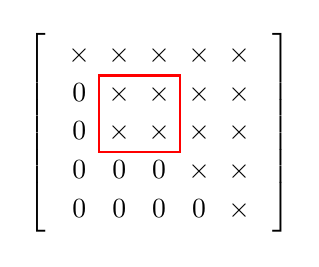
\begin{tikzpicture}
    \matrix[matrix of math nodes,
            nodes in empty cells,
            left delimiter={[},
            right delimiter={]}] (m) 
    {
        \times & \times & \times & \times & \times\\ 
        0      & \times & \times & \times & \times\\
        0      & \times      & \times & \times & \times\\ 
        0      & 0      & 0      & \times & \times\\ 
        0      & 0      & 0      & 0 & \times\\ 
    };

    \draw[red,thick] (m-2-2.north west) rectangle (m-3-3.south east);
\end{tikzpicture}
\end{center}
These Jordan Blocks can easily be solved be taking all such blocks, and then taking the eigenvalues of this sub $2\times 2$ matrix block of all blocks.
Note that the eigenvalues of this block will be a conjugate complex pair.

\section{C implementation}
The implementation written in C can be found at 
\begin{lstlisting}
https://github.com/agamjotsingh1/eigen
\end{lstlisting}

\end{document}
